
P-splines exhibit a number of advantageous properties, many of which are due to the inherited properties of the B-spline basis functions.

\begin{enumerate} \label{eq:PS_properties}
\item \begin{description}\item[Boundary effects]
 P-splines show no boundary effects, as many types of kernel smoothers do. By this, we mean the spreading of a fitted curve or density outside of the (physical) domain of the data, generally accompanied by bending toward zero.
\end{description}
\item \begin{description}\item[P-splines fit polynomial data exactly.] 
P-splines can fit polynomial data exactly. Given data $\left(t_i,y_i\right)$, if the $y_i$ are a polynomial in $t$ of degree $k$, then B-splines of degree $k$ or higher will fit the data exactly. 
\begin{proof}
This statement is equivalent to the claim that given $\xi = \left\{ \xi_i \right\}$, $i=1,\dots,l+1$, and $g$ such that $y\left(t\right) = g\left(t\right)$, we can find an $f \in \PP_{k,\xi} \bigcap \mathscr{C}^{\left(k-2\right)}$ which agrees with $g$ at the points $\tau_1 < \dots < \tau_n$  with $\tau_i \in \left[\xi_1,\xi_{l+1}\right]$ for all $i$, where
\[
n=k+l-1
\]
The solution, $f$ is constructed as follows: generate the knot sequence $t = \left\{t_i\right\}$ as per the recipe in Theorem~\ref{curryschoenbergthm}:
\begin{align*}
t_1 &= t_2 = \dots = t_k = \xi_1 & \\
t_{k+i} &= \xi_{i+1}, & i=1,\dots,l-1\\
t_{n+1} &= t_{n+2} = \dots = t_{n+k} = \xi_{l+1} & 
\end{align*}

Let $\left\{ B_{ik} \right\}$, $i=1,\dots,n$ be the corresponding sequence of B-splines of order $k$, which are a basis for $\PP_{k,\xi} \bigcap \mathscr{C}^{\left(k-2\right)}$ by Theorem~\ref{curryschoenbergthm}. Here, $\PP_{k,\xi} \bigcap \mathscr{C}^{\left(k-2\right)}$ denotes the space of pp functions with breakpoints $\xi$ having two continuous (global) derivatives. Then, \citet{schoenberg1953polya} have shown that there exists exactly one $f \in \PP_{k,\xi} \bigcap \mathscr{C}^{\left(k-2\right)}$ agreeing with $g$ at $\tau_1,\dots, \tau_n$ if and only if 
\[
B_{ik}\left(\tau_i\right) \ne 0, \qquad \qquad i=1,\dots,n.
\]
This $f$ has a unique expansion of the form
\[
f = \sum_{i=1}^n a_i B_{ik}
\] 
for coefficients $a_i,\dots, a_n$, which are the solution to the linear system
\[
\sum_{j=1}^n a_jB_{jk}\left(\tau_i\right) = g\left(\tau_i\right), \qquad \qquad i=1,\dots,n.
\]
This system has a banded matrix of coefficients since $B_{jk}\left(\tau_i\right) \ne 0$ if and only if $\tau_i \in \left[t_j,t_{j+k}\right]$. So if $B_{jk}\left(\tau_i\right) \ne 0$ and thus $\tau_i \in \left(t_j,t_{j+k}\right)$, then there are at most $k$ of the $j$ indices such that $B_{jk}\left(\tau_i\right)$ is nonzero. And further, each of these indices $j$ must be such that 
\[
\left(t_i,t_{i+k}\right) \bigcap \left(t_j,t_{j+k}\right) \ne \emptyset,
\]
or such that $\vert i-j \vert < k$. At worst, the system corresponds to a banded matrix with $k-1$ lower and $k-1$ upper diagonals. 
\end{proof}
The same is true for P-splines if the order of the penalty is $k+1$ or higher, irrespective of the value of $\lambda$. Consider imposing a first-order difference penalty and a fit to data $y$ that is constant - a polynomial of degree 0. Since 
\[
\sum_{j=1}^n \hat{\alpha}_j B_j\left( x_i \right) = c, 
\]
\noindent
we have that
\[
\sum_{j=1}^n \hat{\alpha}_j B^\prime_j\left( x \right) = 0, 
\]
\noindent
for all $x$. From the relationship between differences and derivatives in \ref{eq:more_BS_properties} \ref{eq:BS_deriv_property}, 

\[
0 = \sum_{j=1}^n B^\prime_{j,k}\left(x\right) = \sum_{j=1}^n \Delta\alpha_{j+1} B_{j,k-1}\left( x \right), 
\]
\noindent
so that we must have $\Delta \alpha_j = 0$ for all $j$, and 
\[
\sum_{j=2}^n \Delta \alpha_j = 0.
\]

This shows that the penalty has no impact on the basis coefficients, and the resulting fit is identical to that when using unpenalized B-splines. Using induction, one can show that this is also true when the relationship between $x$ and $y$ is linear and a second order difference penalty is used, and for any values of the polynomial order and order of the difference penalty.\end{description}
\item \begin{description}\item[Null models under difference penalties] \label{eq:PS_property_3}
The limiting P-spline fit approaches a polynomial under strongly enforced smoothing. As $\lambda \rightarrow \infty$, under a difference penalty of order $d$, the fitted function will approach a polynomial of degree $d-1$ as long as the degree of the B-splines is greater than or equal to $k$. To see this, we again need to use the relationship between the differenced coefficient sequence and the derivative of a B-spline as described in \ref{eq:more_BS_properties} \ref{eq:BS_deriv_property}. Consider using the second-order difference penalty; when $\lambda$ is large, the penalty dominates the P-spline objective function defined in \ref{eq:S_pen_varying_intercept_model}, so that the minimizer $\alpha$ must be such that $\sum_{j=3}^n\left(\Delta^2\alpha_j\right)^2$ is close to zero. Consequently, each of the individual second differences must also be nearly zero, and thus the second derivative of the fitted function must be close to zero over the entire domain.
\end{description}
\item \begin{description}\item[The limiting behaviour of $H_\lambda$] The trace of the hat matrix, 
\[
H_\lambda = B\left(B^TB + \lambda D_k^TD_k\right)^{-1}B^Ty
\] 
(or for $H$ defined for the addition of a varying slope component as in \ref{eq:simplest_VC_model_hat_matrix}) approaches $k$, the order of the differencing operator, as $\lambda$ increases. We index $H$ with the smoothing parameter to indicate that the elements of $H$ are a function of $\lambda$. Let
\begin{equation}
Q_B = B^T B \qquad \mbox{and} \qquad Q_\lambda = \lambda D^T D.
\end{equation}
Then using properties of the matrix trace, we can write
\begin{align}
\begin{split}
\mbox{tr}\left(H_\lambda \right) &= \mbox{tr}\bigg[ \left(Q_B + Q_\lambda \right)^{-1}Q_B \bigg]\\
&=\mbox{tr}\bigg[ Q_B^{1/2}\left(Q_B + Q_\lambda \right)^{-1}Q_B^{1/2} \bigg] \\
&=\mbox{tr}\bigg[\left(I + Q_B^{-{1/2}}Q_\lambda Q_B^{-{1/2}} \right)^{-1} \bigg]
\end{split}
\end{align}
Define $L \equiv Q_B^{-{1/2}}Q_\lambda Q_B^{-{1/2}}$. Then
\begin{equation}
\mbox{tr}\left(H_\lambda \right) = \mbox{tr}\bigg[\left(I + \lambda L \right)^{-1} \bigg] = \sum_{j=1}^n \frac{1}{1 + \lambda \gamma_j}
\end{equation}
 where $\gamma_j$, $j=1,\dots,n$ are the eigenvalues of $L$. $Q_\lambda$ has exactly $k$ eigenvalues equal to zero, hence $L$ has $k$ zero eigenvalues. For large $\lambda$, only the $k$ terms with $\gamma_j=0$ contribute to the sum which gives the trace of $H$, so that
 \[
\lim_{\lambda \rightarrow \infty  } \mbox{tr}\left(H\right) = k.
 \]
\end{description}
\end{enumerate}

The previous derivations hold regardless of whether we are fitting the varying intercept-only model, with $\mu\left( t\right) = \beta_0\left(t\right)$ or accommodating a varying slope for a regressor by specifying $\mu\left( t\right) = \beta_0\left(t\right) + \beta_1\left(t\right)x\left(t\right)$. The inspection of the hat matrix $H$ is a prelude to the following section, where we will discuss how to use the properties of $H$ to tune the smoothing parameter for optimal model selection. We will later show that extension of these results can be extended in a rather straightforward manner to the case that is of our particular interest: when the smooth slope function is a two-dimensional surface rather than a curve.

\begin{figure}[H]
\begin{subfigure}{.5\textwidth}
  \centering
   \graphicspath{{img/}}
  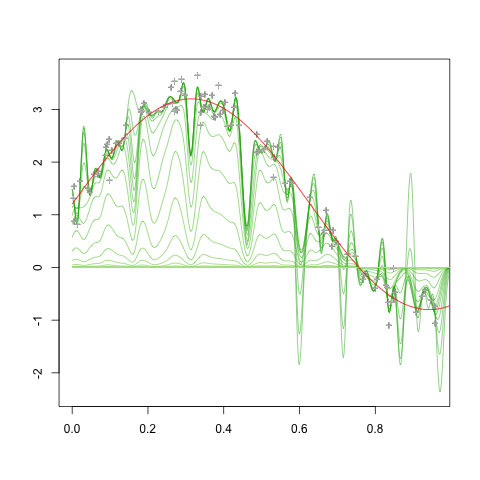
\includegraphics[scale=0.5]{PS_penalty_section_figure_6_order_0.png}
  %\label{fig:pspline_small_lambda}
\caption{$d=0$ }
\end{subfigure}
\begin{subfigure}{.5\textwidth}
  \centering
   \graphicspath{{img/}}
  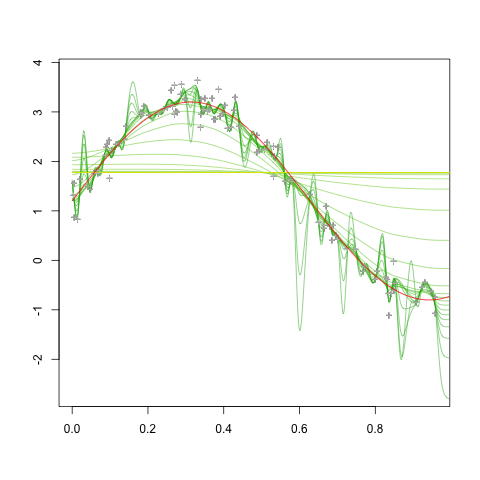
\includegraphics[scale=0.5]{PS_penalty_section_figure_6_order_1.png}
 % \label{fig:pspline_small_lambda}
\caption{$d=1$}
\end{subfigure}
\begin{subfigure}{.5\textwidth}
  \centering
   \graphicspath{{img/}}
  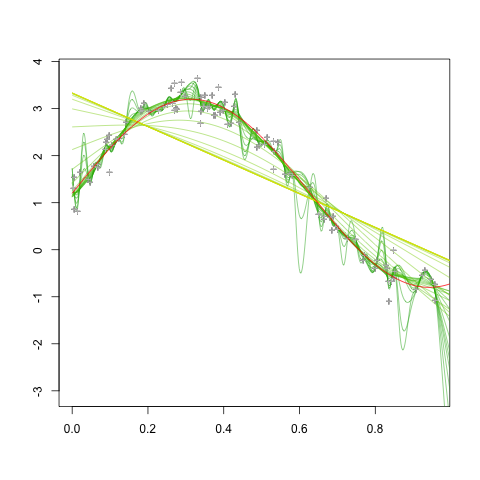
\includegraphics[scale=0.5]{PS_penalty_section_figure_6_order_2.png}
  %\label{fig:pspline_small_lambda}
\caption{$d=2$}
\end{subfigure}
\begin{subfigure}{.5\textwidth}
  \centering
   \graphicspath{{img/}}
  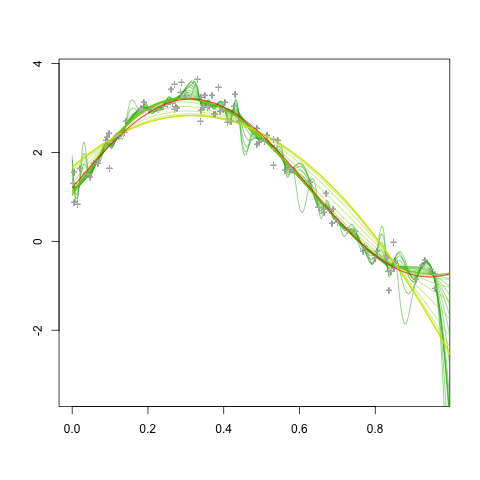
\includegraphics[scale=0.5]{PS_penalty_section_figure_6_order_3.png}
  %\label{fig:pspline_small_lambda}
\caption{$d=3$}
\end{subfigure}
\caption{\textit{Illustration of the impact of the order of the difference penalty. The number of B-splines used is the same in each plot, with the penalty parameter varying from across the same grid of values. The fitted curves in the upper left plot correspond to the difference penalty of order $0$, where $\vert D_0 \alpha \vert^2 = \sum_{i=1}^n \alpha_i^2$, analogous to ridge regression using the B-spline basis as regression covariates. The fitted curves approach polynomials of degree $d-1$ as $\lambda \rightarrow \infty$, as discussed in \ref{eq:PS_properties} \ref{eq:PS_property_3}.}}
\label{fig:PS_penalty_section_figure_6}
\end{figure}

\begin{figure}[h]
\centering
 \graphicspath{{img/}}
  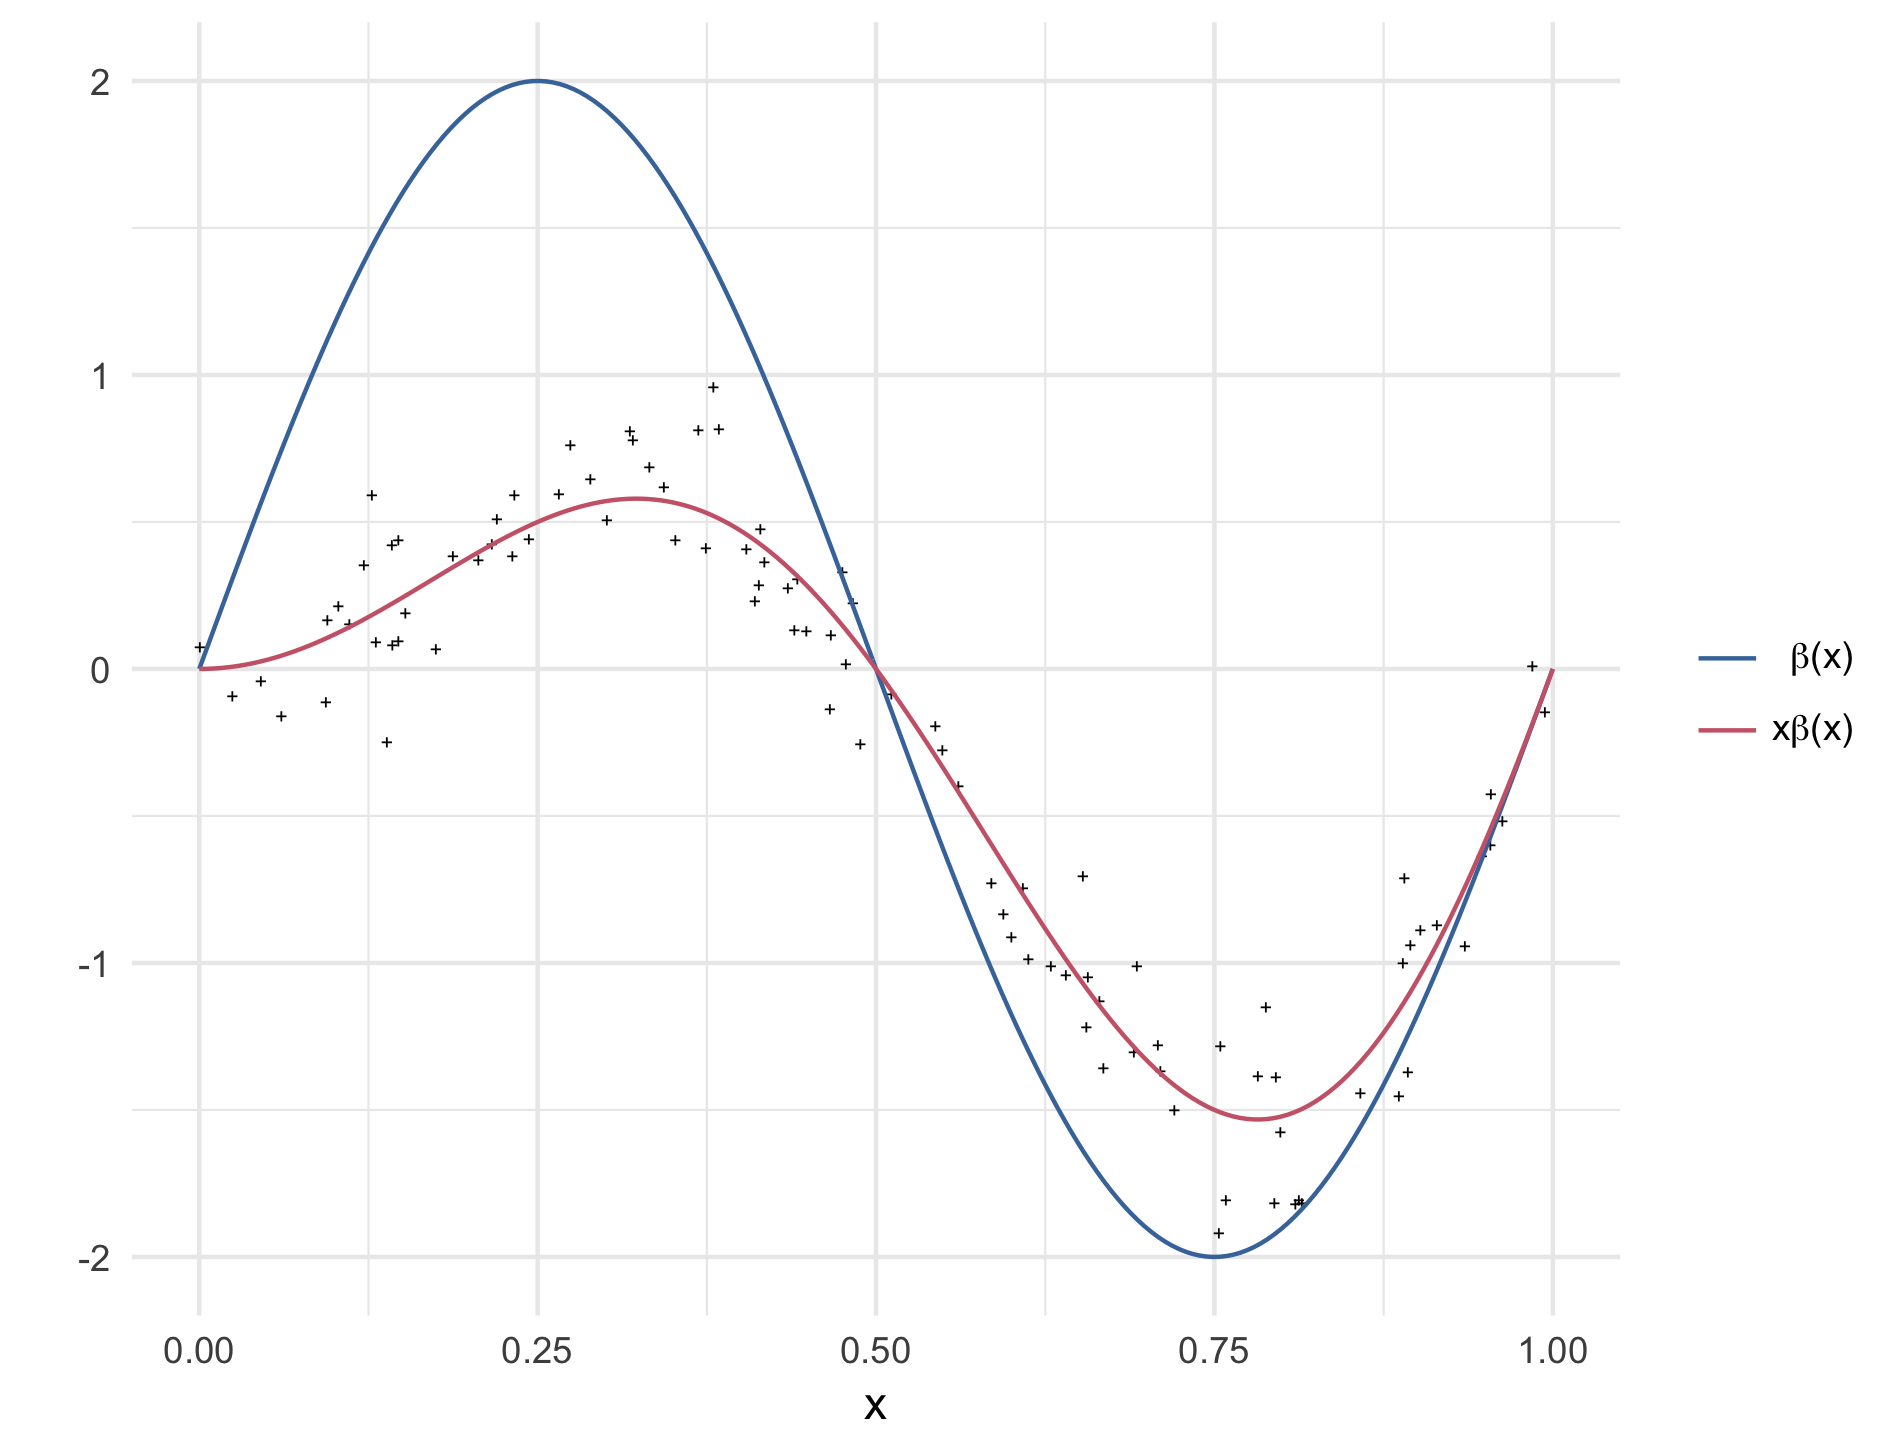
\includegraphics[width=4in, height=4in]{PS_penalty_section_figure_5.png}
 %\caption{Tensor product of two cubic B-splines}
\end{figure}
